\documentclass{llncs}
\usepackage[utf8]{inputenc}

\usepackage{alltt}
\usepackage{url}
\usepackage{graphicx}
\usepackage[percent]{overpic}

\usepackage{xcolor}
\DefineNamedColor{named}{cegla}         {rgb}{.81, .27, .13}
\newcommand{\al}[1]{\textcolor{Peach}{#1}}
\newcommand{\jp}[1]{\textcolor{cegla}{#1}}

\usepackage{hyperref}

\title{Learning to Query: from Concepts in Mind\\to SPARQL Queries}
\author{Jedrzej Potoniec}
\institute{Faculty of Computing, Poznan University of Technology\\ul. Piotrowo 3, 60-965 Poznan, Poland \\\email{Jedrzej.Potoniec@cs.put.poznan.pl}}

\newcommand{\typedliteral}{\textasciicircum\textasciicircum}
\newcommand{\protege}{\emph{Prot\'eg\'e}}

\sloppy

\begin{document}

\maketitle

\begin{abstract}
We present an algorithm learning SPARQL queries reflecting a concept in the mind of a user.
The algorithm leverages SPARQL 1.1 to put most of the complex computations to a SPARQL endpoint.
It operates by building and testing hypotheses expressed as SPARQL queries and uses active learning to collect a small number of learning examples from the user.
We provide an open-source implementation and an on-line interface to test the algorithm.
In the experimental evaluation, we use real queries posed in the past to the official \emph{DBpedia} SPARQL endpoint, and we show that the algorithm is able to learn them, 82\% of them in less than a minute and asking the user just once.
\end{abstract}

\section{Introduction}

Querying data with a complex structure is an inherently hard task for a user.
The user must spend a lot of time learning a vocabulary and relations used in the data.
In this paper, we aim to remedy this issue in context of the data represented as an RDF (Resource Description Framework  \cite{Wood:14:RCA}) graph.

Consider the following use case scenario: a user has a concept in mind, expressed in her own terms.
She knows some of the relevant nodes in the graph, she also knows some of the irrelevant nodes.
Moreover, she can distinguish a relevant node from an irrelevant one for some price, e.g. by spending her time checking it.
She wants to obtain a formal query corresponding to the concept in her mind, to be able to query the graph.

To address this use case, in Section \ref{sec:algorithm} we propose an algorithm for learning a SPARQL \cite{Harris:13:SQL} query by discovering this concept.
The algorithm is designed in such a way that it moves most of the computational work to a SPARQL endpoint by posing quite complex queries to it.
It is a reasonable decision: the RDF graph is stored there, so it is the best place to perform any optimization.
A few years ago it would not work, but recent increase in computational power and development of RDF stores made it feasible.

Thought this work, we use the following prefixes: \texttt{dbr:} for \url{http://dbpedia.org/resource/}, \texttt{dbo:} for \url{http://dbpedia.org/ontology/}, \texttt{dbp:} for \url{http://dbpedia.org/property/}, \texttt{dct:} for \url{http://purl.org/dc/terms/}, \texttt{xsd:} for \url{http://www.w3.org/2001/XMLSchema#}.

\section{Related work}

For the past few years, researchers proposed many approaches for querying an RDF graph alternative to writing a formal query by hand.
Roughly, they can be divided into a few categories: faceted browsing, natural language interfaces, visual interfaces and recommendations.
In faceted browsing a user is presented with an interface dynamically generated from an RDF graph to filter the graph according to her needs, e.g. see \cite{DBLP:conf/semweb/OrenDD06}.
Also variants tailored to a specific types of data were proposed, e.g. \cite{leon2012map4rdf} describes an interface for geospatial data.
A recent system \emph{Sparklis} \cite{DBLP:conf/semweb/Ferre14a} combines faceted browsing with natural language generation to enable a non-expert user to query an RDF graph.

Natural language interfaces are concerned with answering a query specified in a natural language, e.g. by translating it to SPARQL and then posing it to an endpoint.
These systems are frequently tailored to some specific task and/or a specific RDF graph.
For example, \emph{Xser} \cite{DBLP:conf/clef/XuFZ14} is a system for answering factual questions and \emph{CubeQA} \cite{DBLP:conf/i-semantics/HoffnerL14} is designed to answer statistical queries requiring aggregate functions.
A very recent survey \cite{hoffner2016survey} gives a comprehensive overview of such systems.

The visual interfaces offer a possibility of constructing a query by visual means, e.g. by navigating over a displayed part of a graph \cite{DBLP:conf/semweb/ZainabSMZDH15} or by constructing a SPARQL query from building blocks \cite{DBLP:conf/semweb/BottoniC15}.

A system using recommendations still requires from a user knowledge of SPARQL, but it helps to deal with an unknown vocabulary.
\cite{DBLP:conf/hci/GombosK14} recommends predicate names based on an inferred type of a variable in a triple pattern.
\cite{DBLP:conf/dexaw/CampinasPCDT12} describes a method for recommending query terms based on a graph summary, while \cite{DBLP:conf/semweb/Campinas14} pushes it even further by performing the recommendations on-line, by posing appropriate queries to a SPARQL endpoint.

A similar idea to ours was already proposed in \cite{DBLP:conf/esws/LehmannB11}.
The main difference are the assumptions: \cite{DBLP:conf/esws/LehmannB11} performs all the computation on the client-side, obtaining information about resources using an approach similar to Concise Bounded Description \cite{cbd} and then computing their intersections.
Our approach leverages new features of SPARQL 1.1 and thus moves most of the learning complexity directly to a SPARQL endpoint.

Methods for learning queries from a set of examples were also discussed in other contexts.
\cite{DBLP:journals/ijswis/LawrynowiczP14} uses a pattern mining approach to learn a set of SPARQL queries, which then are used as binary patterns for a normal classification algorithm.
In \cite{DBLP:conf/wims/PaulheimF12} the authors propose a method for unsupervised mining of data mining features, which directly correspond to SPARQL queries.
\cite{DBLP:journals/jmlr/Lehmann09} and \cite{DBLP:conf/ilp/FanizzidE08} are methods for learning Description Logics class expressions from a set of positive and negative examples.
The expressions can then be used as queries to an ontological knowledge base to retrieve individuals fulfilling the class expression, e.g. using a \emph{DL Query} tab of \protege{} \cite{DBLP:journals/ijmms/GennariMFGCENT03}.

\section{Learning SPARQL queries\label{sec:algorithm}}

\subsection{Basic concepts}

Throughout this section, we use the following example: the user wants to formulate a SPARQL query which allows her to query \emph{DBpedia} \cite{DBLP:conf/semweb/AuerBKLCI07} for the capitals of states of the European Union.
She knows some of them: Warsaw, Berlin, Zagreb, Nicosia and Vilnius.
She can also recognize if an arbitrary DBpedia URI refeers to one of the capitals by reading a Wikipedia article corresponding to the URI.
Of course, reading consumes her time, so she wants to limit the number of articles read.
She also know that Oslo, being a capital of Norway, which is not an European Union member, should not be present in the results.

In a very broad terms, the algorithm works by formulating a hypothesis and verifying it with the user.
A \emph{hypothesis} consists of SPARQL triple patterns and filters.
Every triple pattern in the hypothesis has a fixed predicate (i.e. the predicate is an URI), the subject and object may be an URI, a literal or a variable.
Every filter contains only an expression of form \emph{variable \texttt{>=} fixed literal} or \emph{variable \texttt{<=} fixed literal}.
An \emph{empty hypothesis} is a hypothesis, which contains no triple patterns or filters.
We require that an undirected graph corresponding to a basic graph pattern defined by a hypothesis is a connected graph.
A \emph{query corresponding to a hypothesis} is a SELECT SPARQL query with a single variable in the head.
We ask only for unique bindings, i.e. the variable is preceded with DISTINCT modifier.
The WHERE clause contains only the hypothesis and there are no other clauses in the query.
We denote a hypothesis by \texttt{H(?uri)}, where \texttt{?uri} is the variable in the head of the corresponding query.
For example, the algorithm may generate the following hypothesis \texttt{H(?uri)}:
\begin{alltt}
dbr:European_Union dbo:wikiPageWikiLink ?uri .
?uri dct:subject dbr:Category:Capitals_in_Europe .
dbr:Member_state_of_the_European_Union dbo:wikiPageWikiLink ?uri.
\end{alltt}

To formulate a hypothesis, the algorithm uses a set of positive examples \texttt{P} and a set of negative examples \texttt{N}.
Both of these sets contain URIs from the RDF graph.
\texttt{P} is a subset of URIs expected in the results of the final hypothesis.
\texttt{N} is a set of URIs which are forbidden to appear in these results.
They do not need to be fully specified before the algorithm is run, instead it is enough that the user provides a few URIs in both sets, and then they are extended during the execution of the algorithm.
\texttt{n\_pos} stands for the number of URIs in the set \texttt{P}.
In our running example, \texttt{P} initially consists of \texttt{dbr:Warsaw}, \texttt{dbr:Berlin}, \texttt{dbr:Zagreb}, \texttt{dbr:Nicosia} and \texttt{dbr:Vilnius}, and thus $\texttt{n\_pos}=5$.
\texttt{N} contains only \texttt{dbr:Oslo}.

The algorithm uses well-known information retrieval measures.
Denote by $TP$ a number of URIs from the set \texttt{P} which were retrieved by a hypothesis, and by $FP$ a number of URIs from the set \texttt{N} which were retrieved by the hypothesis.
Following \cite{mir2e}, we define three measures.
\emph{Precision} is a fraction of positive URIs retrieved by the hypothesis over both positive and negative URIs retrieved by the hypothesis, i.e. $p=\frac{TP}{TP+FP}$.
\emph{Recall} is a fraction of positive URIs retrieved by the hypothesis over the number of known positive URIs \texttt{n\_pos}, i.e. $r=\frac{TP}{\texttt{n\_pos}}$.
Finally, \emph{$F_1$ measure} is a harmonic mean of precision and recall, i.e. 
\[F_1 = \frac{2}{\frac{1}{p}+\frac{1}{r}}\]

\subsection{Overview of the algorithm\label{sec:overview}}

In the beginning of the algorithm, the user is asked to provide a few positive and a few negative examples.
The hypothesis considered by the algorithm is set to an empty hypothesis.
The hypothesis is then refined, as described in the Section \ref{sec:refinement}.
Then, the algorithm generates a few examples that follow the hypothesis and a few examples that contradict the hypothesis, and the user is asked to assign them to one of the two sets.
If any of the examples following the hypothesis is assigned to the set \texttt{N}, it means that the hypothesis is invalid and the last refinement is retracted.
If the hypothesis is good enough w.r.t. the known examples (c.f. Section \ref{sec:goodenough}), it is presented to the user along with the full result of posing it to the SPARQL endpoint.
The user then must either accept the hypothesis or add at least one new positive or negative example, e.g. by selecting a URI from the result which should not be there, or by adding a URI which is missing.
If the hypothesis is not good enough or the user adds a new example, the algorithm goes back to generating a new refinement.

\subsection{Measuring quality of a hypothesis \label{sec:goodenough}}

To compute with a SPARQL endpoint how good a hypothesis is, the following query is used:
\begin{alltt}
SELECT (COUNT(DISTINCT ?s) as ?tp) (COUNT(DISTINCT ?t) AS ?fp) 
        (?tp/(?tp+?fp) AS ?precision) (?tp/n_pos AS ?recall)
        (2/((1/?precision)+(1/?recall)) AS ?f1)
WHERE \{
    \{
        H(?s)
        VALUES ?s \{ P \}
    \} UNION \{
        H(?t)
        VALUES ?t \{ T \}
    \}\}
\end{alltt}
Such a query computes the measures described above.
The variable \texttt{?s} (resp. \texttt{?t}) is bound to all URIs from the set \texttt{P} (resp. \texttt{N}) that follow the hypothesis, thus \texttt{?tp} corresponds to $TP$, \texttt{?fp} to $FP$ and so on.
If the value of $F_1$ measure is high enough, the hypothesis is \emph{good enough} w.r.t to the examples available to the algorithm, and it is presented to the user as a final answer.

\subsection{Generating new examples and querying the user\label{sec:new_examples}}

If the hypothesis is not good enough, the algorithm should gather more evidence, to either confirm or reject it.
To do so, the algorithm must generate a small set of examples that follow the hypothesis and another small set of examples that contradicts the hypothesis.
To generate examples following the hypothesis, the following query is used:
\begin{alltt}
SELECT DISTINCT ?uri
WHERE \{
    H(?uri)
    FILTER(?uri NOT IN (P N))
\} LIMIT 3
\end{alltt}
\texttt{H(?uri)} in the query ensures that an example follows the hypothesis, and \texttt{FILTER} ensures that it is a new example, i.e. one that is not present in either of the sets \texttt{P} and \texttt{N}.
\texttt{LIMIT 3} is to ensure that we query the user only about a small number of new examples.
Recall the example and let \texttt{H(?uri)} be \texttt{dbr:European\_Union dbo:wikiPageWikiLink ?uri.} Possible new examples are \texttt{dbr:Above\_mean\_sea\_level}, \texttt{dbr:Afroasiatic\_languages}, \texttt{dbr:Andorra}, neither of them following the concept we aim for, as the hypothesis is too broad.

Generating negative examples is more difficult.
Let \texttt{Hp(?uri)} be a hypothesis the hypothesis \texttt{H(?uri)} directly originated from, i.e. \texttt{Hp(?uri)} is the hypothesis \texttt{H(?uri)} without the last refinement.
Consider the following SPARQL query:
\begin{alltt}
SELECT DISTINCT ?uri
WHERE \{\{
        \{ Hp(?uri) \}
        MINUS
        \{ H(?uri) \}
    \} FILTER(?uri NOT IN (P N))
\} LIMIT 3
\end{alltt}
The only common variable between \texttt{Hp(?uri)} and \texttt{H(?uri)} is \texttt{?uri}, the rest is uniquely renamed.
This query provides a set of examples that follow the hypothesis except for the last refinement.
\texttt{FILTER} and \texttt{LIMIT} are used for the same purpose as before.
The process of generating new examples follows the idea of active learning, where a learning algorithm selects unknown examples to maximize benefit from getting correct labels for them, e.g. to remove as much uncertainty as possible \cite{Cohn2010}.

After the examples are generated, they are presented to the user.
She must then assign each of them either to the set \texttt{P} or \texttt{N}.
After the assignment is done, the algorithm continues, as described in Section \ref{sec:overview}.

\subsection{Hypothesis refinement\label{sec:refinement}}

If the hypothesis is not good enough, the algorithm must refine it.
First, the algorithm checks if it is possible to generate new examples using the current hypothesis.
If not, the most recent refinement of the hypothesis is retracted and the condition is checked again.
The process continues until it becomes possible to generate new examples.
In the worst case, it means emptying the hypothesis.

To refine the hypothesis, the algorithm must generate a set of possible refinements and select the best of them.
First, consider a refinement consisting of a single triple pattern with a fixed predicate and object, and a subject being a variable already present in the hypothesis.
For example, such a refinement could be \texttt{?uri dct:subject dbr:Category:Capitals\_in\_Europe}.
To generate a set of such refinements the following query is used.
\begin{alltt}
SELECT ?p ?o (COUNT(DISTINCT ?s) AS ?tp) (COUNT(DISTINCT ?t) AS ?fp) 
        (?tp/(?tp+?fp) AS ?precision) (?tp/n_pos AS ?recall)
        (2/((1/?precision)+(1/?recall)) AS ?f1)
WHERE \{\{
        H(?s)
        ?s ?p ?o .
        VALUES ?s \{ P \}
    \} UNION \{
        H(?t)
        ?t ?p ?o .
        VALUES ?t \{ N \}
    \}\}
GROUP BY ?p ?o
HAVING (?recall>=.99)
\end{alltt}
Observe, that the results are grouped by the pair \texttt{?p ?o}, so effectively what this query does is to compute the measures for a lot of hypotheses at once, each consisting of the original hypothesis $H$ and a refinement with a subject being a variable already present in the hypothesis (\texttt{?s} and \texttt{?t}) and fixed values for a predicate and an object.
We require for the recall to reach at least $0.99$, to ensure that all known positive examples are covered by a new hypothesis.

Recall the example, and let \texttt{H(?uri)} be \texttt{dbr:European\_Union dbo:wikiPageWikiLink ?uri.}
A refinement \texttt{?uri dct:subject dbr:Category:Capitals\_in\_Europe .} has recall $r=1$, as it returns all five elements of the set \texttt{P}, and it also has precision $p=1$ as it does not return the negative example, i.e. Oslo.
On the other hand, a refinement \texttt{?uri dbo:utcOffset "+2"} will not be considered, as its recall is 0.8 (\texttt{dbr:Berlin} does not occur in such a triple).

To compute refinements with a fixed subject, but a variable object, the algorithm uses the same query, but replaces \texttt{?s ?p ?o} (resp. \texttt{?t ?p ?o}) with \texttt{?o ?p ?s} (resp. \texttt{?o ?p ?t}).
Finally, to compute refinements with a fixed predicate, a new variable as an object (resp. subject) and an existing variable as a subject (resp. object), the algorithm replaces \texttt{?o} with a blank node \texttt{[]} in the triple patterns and removes \texttt{?o} from the head and from the GROUP BY clause.

It requires a more elaborate query to provide refinements with FILTER.
Consider the following query:
\begin{alltt}
SELECT ?p ?l (COUNT(DISTINCT ?s) AS ?tp) (COUNT(DISTINCT ?t) as ?fp)
    (?tp/(?tp+?fp) AS ?precision) (?tp/n_pos AS ?recall)
    (2/((1/?precision)+(1/?recall)) AS ?f1)
WHERE \{\{
        H(?s)
        ?s ?p ?xl. FILTER(isLiteral(?xl))
        VALUES ?s \{ P \}
    \} UNION \{
        H(?t)
        ?t ?p ?xl. FILTER(isLiteral(?xl))
        VALUES ?t \{ N \}
    \} FILTER(?xl <= ?l) \{
        SELECT DISTINCT ?p ?l
        WHERE \{
            H(?s)
            ?s ?p ?l. FILTER(isLiteral(?l))
            VALUES ?s \{ P \}
        \}\}\}
GROUP BY ?p ?l
HAVING (?recall >= .99)
\end{alltt}
The query operates in two steps.
First, the subquery extracts all pairs consisting of a predicate \texttt{?p} and a literal \texttt{?l} for the set \texttt{P}.
Then, for every pair \texttt{?p ?l} it computes the measures for a hypothesis consisting of the original hypothesis \texttt{H(?s)}, a triple pattern \texttt{?s ?p ?xl} (\texttt{?xl} is a new variable), and a filter comparing the new variable \texttt{?xl} to a literal \texttt{?l} from the subquery.
Again, we require the recall to be at least $0.99$ to ensure appropriate coverage of positive examples.
An example of a refinement obtained this way is
\texttt{?uri dbo:populationTotal ?var1337. filter(?var1337 >= "205934"\typedliteral xsd:nonNegativeInteger).}

When the set of the possible refinements is collected from the endpoint, the algorithm must choose the right one.
The set of refinements is sorted according to descending values of the $F_1$ measure and (in case of ties on $F_1$) the precision.
For every refinement, the algorithm checks if the current hypothesis with the refinement added is good enough.
If it is, the hypothesis is displayed to the user, as described in Section \ref{sec:overview}.
Otherwise, the algorithm tries to generate new positive and negative examples (c.f. Section \ref{sec:new_examples}).
If it is not possible, the refinement is retracted from the hypothesis and the next refinement in order is checked.
If the examples were generated, the algorithm proceeds as described earlier.
If the algorithm fails to find any suitable refinement, it terminates with a failure.

\section{Implementation\label{sec:impl}}

To make it easier to reuse the algorithm, we provide a \emph{Python} implementation of the algorithm available in  a \emph{Git} repository: \url{https://bitbucket.org/jpotoniec/kretr/}.
We also developed an on-line interface to the implementation which we coupled with \emph{Blazegraph 2.1.1}\footnote{\url{https://www.blazegraph.com/}} loaded with \emph{DBpedia 2015-04} and made publicly accessible at  \url{https://semantic.cs.put.poznan.pl/ltq/}.
In the implementation, we assume a hypothesis to be good enough if the $F_1$ measure is at least $0.99$.
Screenshots of the interface are presented in Figures \ref{fig:sc1} and \ref{fig:sc2}.

\begin{figure}
\centering
%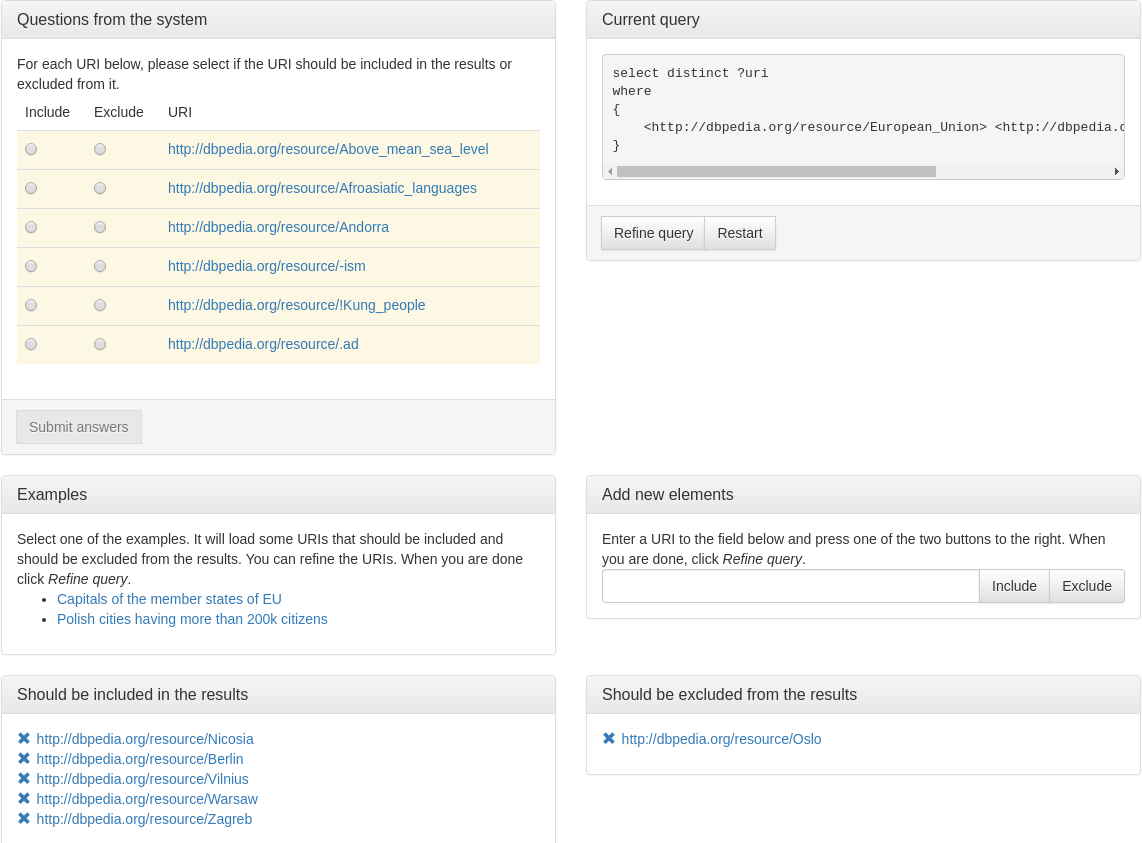
\includegraphics[width=\textwidth]{sc1.png}
\begin{overpic}[width=\textwidth,tics=10]{sc1.png} %grid,
 \put (90,65) {\huge 1}
 \put (40,50) {\huge 2}
 \put (25,5) {\huge 3}
 \put (75,5) {\huge 4}
 \put (80,20) {\huge 5}
 \put (35,19) {\huge 6}
\end{overpic}
\caption{A screenshot of the on-line interface to the implementation of the algorithm.
It presents (1) the query corresponding to a current hypothesis, (2) a set of new examples the user is supposed to assign to one of the two sets and already known (3) positive, and (4) negative examples.
It is also possible to (5) add a new example by entering its URI or (6) load one of the demo scenarios.
}
\label{fig:sc1}
\end{figure}

\begin{figure}
\centering
\begin{overpic}[width=\textwidth,tics=10]{sc2.png} 
 \put (35,15) {\huge 2}
 \put (80,22) {\huge 1}
 \put (-1,10) {\huge 3}
 \put (55,2) {\huge 4}
\end{overpic}
\caption{After a good enough hypothesis is reached, the interface displays (1) the query corresponding to the hypothesis and (2) results of posing it to the SPARQL endpoint.
The user can then use (3) the \texttt{X} buttons to remove some of the unwanted results and further (4) refine the query.}
\label{fig:sc2}
\end{figure}

\section{Experimental evaluation}

To validate the algorithm, we posed the following research question: is the algorithm able to cover requirements of real users of \emph{DBpedia}?
To answer the question, we collected a set of SPARQL queries from the logs of the official \emph{DBpedia} SPARQL endpoint and used the queries as a gold standard.
The queries and the raw results of the experiment are available in the repository with the source code (see Section \ref{sec:impl}).
Below, we describe the details of the experiment.

\subsection{Setup}

The \emph{Linked SPARQL Queries} dataset contains queries obtained from query logs of SPARQL endpoints for various popular Open Linked Data datasets  \cite{DBLP:conf/semweb/SaleemAHMN15}.
Among others, it contains queries from the official \emph{DBpedia} SPARQL endpoint, for the period from 30.04.2010 to 20.07.2010.
From this set, we selected queries that are SELECT queries and contain only a single variable in the head or use star in the head, but contain only a single variable.
This way we obtained 415342 queries (415145 character-wise distinct queries).
We then randomly selected 50 queries, which did not fail when posed to a \emph{DBpedia} SPARQL endpoint and resulted in at least 20 different URIs.
The endpoint run on \emph{Blazegraph 2.1.1} and contained \emph{DBpedia} 2015-04.
For the selected 50 queries, the smallest number of different URIs was 20, and the largest 2060507.

For each of the selected queries, we used it to simulate a user.
The query was posed to the SPARQL endpoint and its results (any duplicates removed) were used as a gold standard, i.e. a set of all URIs the simulated user is interested in.
Out of the gold standard, we randomly selected 5 URIs, which were given to the algorithm as initial positive examples.
To provide negative examples we randomly selected the following six URIs: \texttt{dbr:Bydgoszcz, dbr:Murmur\_\%28record\_label\%29, dbr:Julius\_Caesar, dbo:abstract, dbp:after, dbo:Agent}.
If any of these negative examples was in the gold standard, it was removed from the set of negative examples.

We then run the algorithm until it converged to a hypothesis that resulted in exactly the same set of URIs as the gold standard, or for 10 good enough hypotheses generated by the algorithm, whatever came first.
If a good enough hypothesis was not perfect, we randomly added up to 5 new positive examples (i.e. new URIs which were present in the gold standard, but were not present in the results of the hypothesis) and up to 5 new negative examples (i.e. new URIs that were present in the results of the hypothesis, but were not present in the gold standard).
We also counted number of interactions of the simulated user with the algorithm and measured wall time.

\subsection{Results}

For 41 of the selected queries the first good enough hypothesis presented to the simulated user was perfect, for 8 the second, and for 1 only the third hypothesis was perfect.
The WHERE clause of the gold standard query corresponding to this last case was
\texttt{?value dbp:subdivisionType dbr:List\_of\_counties\_in\_Montana.}
The first hypothesis was too broad, consisting of only \texttt{?uri dbp:areaCode "406"\typedliteral{}xsd:integer.}
Apparently, this is a correct telephone area code for the state of Montana \cite{wiki:montana}, but so it is for Gümüşhane Province in Turkey \cite{wiki:turkey}.
The second try was, on the other hand, too narrow:
{
\small
\begin{alltt}
?uri dbp:subdivisionType dbr:Political_divisions_of_the_United_States .
?uri dbp:subdivisionType dbr:List_of_counties_in_Montana .
\end{alltt}
}
It omitted four resources from the gold standard: \texttt{dbr:Browning,\_Montana}, \texttt{dbr:Missoula,\_Montana}, \texttt{dbr:Great\_Falls,\_Montana}, \texttt{dbr:Helena,\_Montana}.
After they were added as positive examples, the algorithm converged to the correct hypothesis.

For 38 of the queries, the simulated user was asked only once to label a set of six examples, in case of 4 queries the user was asked twice, for 3 queries thrice, for 2 queries four times, for another 2 queries five times and a once six times.
The user waited on average for $56\pm 22$ seconds (median: 41 seconds) during the whole process for the algorithm to generate new examples or present a good enough hypothesis.
In case of queries which reached the gold standard with the first good enough hypothesis, the average time was $50\pm 2$ seconds.
For $82\%$ of the queries the user obtained a perfect hypothesis in less than a minute and was asked to label at most 12 examples. 
That means the algorithm is really able to cover requirements of the users, it does not waste their time in waiting and we can answer positively to the research question.



\section{Conclusions}

We presented an algorithm for learning SPARQL queries reflecting a concept in mind of a user using examples provided by the user.
The algorithm uses active learning to minimize required number of examples.
It is also suitable for any RDF graph accessible through a SPARQL endpoint and does not require any preprocessing or initialization phase.
SPARQL 1.1 gave us a set of powerful tools, which enabled us to move most of the complex computations in the algorithm to the SPARQL endpoint.
Contemporary RDF stores (e.g. \emph{Blazegraph}) are very sophisticated and are able to deal with such queries without any problem.
To prove that the algorithm works, we provide an on-line interface for testing, available at \url{https://semantic.cs.put.poznan.pl/ltq/}.
We also performed an experiment using real queries obtained from the \emph{Linked SPARQL Queries}. We showed that the algorithm is able to converge to a gold standard with only a minimal amount of interaction with the user.

In the future, we would like to analyze if using different measures may provide even faster convergence to a correct hypothesis.
We would also like to extend the algorithm with possibility of obtaining some prior knowledge from the user.
Finally, this algorithm is targeted for an end-user, who is not necessarily a Semantic Web expert.
Coupling the algorithm with a tool for visual presentation of SPARQL queries and displaying \emph{Wikipedia} links instead of \emph{DBpedia} URIs would enable us to perform a crowdsourcing experiment to verify if the algorithm meets the requirements of non-expert users.

\subsubsection*{\ackname}
Jedrzej Potoniec acknowledges support of Polish National Science Center, grant DEC-2013/11/N/ST6/03065.

\bibliographystyle{splncs03}
\bibliography{main}


\end{document}
